\documentclass[final]{siamltex}
%test change
\usepackage{cite}
\usepackage{graphicx,bbm,pstricks}
\usepackage{pifont}
\usepackage{bbm,algorithmic,mdframed,placeins,multirow,booktabs}
\setlength{\parindent}{0in}
\usepackage{amsmath,amsfonts,amsbsy}
\newcommand{\RARR}[3]{#1
  \;\displaystyle\mathop{\displaystyle\longrightarrow}^{#3}\; #2}
\newcommand{\RARRlong}[3]{#1
  \;\displaystyle\mathop{-\!\!\!-\!\!\!-\!\!\!-\!\!\!-\!\!\!\!\displaystyle
  \longrightarrow}^{#3}\; #2}
\newcommand{\LARR}[3]{#1
  \;\displaystyle\mathop{\displaystyle\longleftarrow}^{#3}\; #2}
\newcommand{\LRARR}[4]{{\mbox{ \raise 0.4 mm \hbox{$#1$}}} \;
  \mathop{\stackrel{\displaystyle\longrightarrow}\longleftarrow}^{#3}_{#4}
  \; {\mbox{\raise 0.4 mm\hbox{$#2$}}}}
\newcommand{\bX}{{\bf X}}
\newcommand{\vecx}{{\mathbf x}}
\newcommand{\vecy}{{\mathbf y}}
\newcommand{\vecz}{{\mathbf z}}
\newcommand{\vecq}{{\mathbf q}}
\newcommand{\bs}{{\mathbf s}}
\newcommand{\vecr}{{\mathbf r}}
\newcommand{\vecX}{{\mathbf X}}
\newcommand{\vecv}{{\mathbf v}}
\newcommand{\tick}{\ding{52}}
\newcommand{\cross}{\ding{54}}
\newcommand{\vecn}{{\mathbf n}}
\newcommand{\vecp}{{\mathbf p}}
\newcommand{\cT}{{\mathcal T}}
\newcommand{\dt}{{\mbox{d}t}}
\newcommand{\dx}{{\mbox{d} \vecx}}
\newcommand{\boldnu}{{\boldsymbol \nu}}
\newcommand{\er}{{\mathbb R}}
\renewcommand{\div}{{\rm div}}
\newcommand{\bnu}{{\bf \nu}}
\newcommand{\divergence}{\mathop{\mbox{div}}}
\renewcommand{\P}{\mathbb{P}}
\newcommand{\FP}{P_{\rm{FP}}}
\newcommand{\ME}{P_{\rm{ME}}}
\newcommand{\MEs}{P_{\rm{ME}_{S}}}
\newcommand{\D}{\mathcal{D}}
\newcommand{\G}{\mathcal{G}}
\newcommand{\N}{\mathcal{N}}
\newcommand{\X}{{\mathbf X}}
\newcommand{\Y}{{\mathbf Y}}
\newcommand{\W}{{\mathbf W}}
\newcommand{\data}{D}
\newcommand{\neff}{n_{\text{eff}}}
\newcommand{\E}{{\mathbb E}}

\newcommand{\picturesAB}[6]{
\centerline{
\hskip #4
\raise #3 \hbox{\raise 0.9mm \hbox{(a)}}
\hskip #5
\epsfig{file=#1,height=#3}
\hskip #6
\raise #3 \hbox{\raise 0.9mm \hbox{(b)}}
\hskip #5
\epsfig{file=#2,height=#3}
}}
\newcommand{\picturesCD}[6]{
\centerline{
\hskip #4
\raise #3 \hbox{\raise 0.9mm \hbox{(c)}}
\hskip #5
\epsfig{file=#1,height=#3}
\hskip #6
\raise #3 \hbox{\raise 0.9mm \hbox{(d)}}
\hskip #5
\epsfig{file=#2,height=#3}
}}
\author{Colin Cotter\thanks{Department of Mathematics, Imperial
    College, London, UK} \and Simon Cotter\thanks{School of
    Mathematics, University of Manchester, Manchester, UK. e: simon.cotter@manchester.ac.uk} \and Paul Russell\thanks{School of
    Mathematics, University of Manchester, Manchester, UK}}
\title{Parallel Adaptive Importance Sampling}
\begin{document}
\maketitle
\begin{abstract}
  Markov chain Monte Carlo methods are a powerful and commonly used
  family of numerical methods for sampling from complex probability
  distributions. As applications of these methods increase in size and complexity, the need for efficient
  methods which can exploit the parallel architectures which are
  prevalent in high performance computing increases. In this paper, we
  aim to develop a framework for scalable parallel MCMC algorithms. At
  each iteration, an importance sampling proposal distribution is
  formed using the current states of all of the chains within an
  ensemble. Once weighted samples have been produced from this, a
  state-of-the-art resampling method is then used to create an evenly
  weighted sample ready for the next iteration. We demonstrate that
  this parallel adaptive importance sampling (PAIS) method outperforms
  naive parallelisation of serial MCMC methods using the same number
  of processors, for low dimensional problems, and in fact shows
  better than linear improvements in convergence rates with respect to
  the number of processors used.
\end{abstract}
\begin{keywords}MCMC, parallel, importance sampling, Bayesian, inverse problems.
\end{keywords}
\section{Introduction}
%\subsection{Lit. review}
%\subsection{Optimal transport resampler}
%\subsection{Function Space MCMC}
Markov chain Monte Carlo (MCMC) methods are a powerful family of tools
that allow us to sample from complex probability distributions. MCMC
methods were first developed in the 70s\cite{hastings1970monte}, and with the development of
to use MCMC methods for many more. In particular, when
considering Bayesian inverse problems, each MCMC step may involve the
numerical solution of one or more PDE. As many samples are usually
required before Monte Carlo error is reduced to acceptable levels,
these types of problem remain frustratingly out of our grasp.

Many advances have been made in the field of MCMC to design ever more
complex methods that propose moves more intelligently, leading to
rapidly converging methods. Function space versions of standard methods
such as the random walk Metropolis-Hastings (RWMH) algorithm or the
Metropolis adjusted Langevin algorithm (MALA), whose convergence rates
are independent of dimension have been
developed\cite{cotter2013mcmc}. The hybrid (or Hamiltonian) Monte
Carlo (HMC) method uses Hamiltonian dynamics in order to propose and
accept moves to states which are a long way away from the current
position\cite{sexton1992hamiltonian}, and function space analogues of
this have also been proposed\cite{beskos2011hybrid}. Riemann
manifold Monte Carlo methods exploit the Riemann geometry of the
parameter space, and are able to take advantage of the local structure
of the target density to produce more efficient MCMC
proposals\cite{girolami2011riemann}. This methodology has been
successfully applied to MALA-type proposals and methods which exploit
even higher order gradient information\cite{bui2014solving}.  These
methods allow us explore the posterior distribution more fully 
with fewer iterations.

Simultaneously, great strides are continually being made in the
development of computing hardware. Moore's law, which predicted that
the number of transistors that can to fit on a single microchip will
double every two years, has been largely followed since the early
70s\cite{moore1998cramming}. In recent times, it has become necessary
to use parallel architectures to exploit Moore's law. The efficient
exploitation of these facilities is the key to solving many of the
computational challenges that we currently face.

As such, the development of efficient parallel MCMC algorithms is an
important area for research. Since MCMC methods can be trivially
parallelised by simply running many independent chains in parallel,
the focus needs to be on the development of methods which gain some
added benefit through parallelism. One class of parallel MCMC method
uses multiple proposals, with only one of these proposals being
accepted. Examples of this approach include multiple try
MCMC\cite{liu2000multiple} and ensemble MCMC\cite{neal2011mcmc}. In
\cite{calderhead2014general}, a general construction for the
parallelisation of MCMC methods was presented, which demonstrated
speed ups of up to two orders of magnitude when compared with serial methods.

In this paper, we present a framework for parallelisation of
importance sampling, which can be built around any of the current
Metropolis-based methodologies in order to create an efficient target
proposal from the current state of all of the chains in the
ensemble. The idea is to consider the parallel chains as an ensemble,
and to resample using a transformation based on optimal transport.
Samplers based on optimal transport have also been considered in
\cite{el2012bayesian}.

In Section \ref{Sec:Prelim} we outline some preliminaries,
including the general set up for Bayesian inverse problems, the
preconditioned Crank-Nicolson Langevin (pCNL) algorithm and a
brief review of the optimal transport resampler,  both of which we will be
employing within the algorithm. We describe the Parallel Adaptive
Importance Sampler (PAIS) in Section \ref{Sec:PAIS}, and in Section
\ref{Sec:adapt} we describe how algorithmic parameters can be
automatically tuned to provide optimal convergence. In
Section \ref{Sec:Num}, we present some numerical experiments that
demonstrate the savings available by employing this approach as
opposed to a naive/trivial parallelisation of existing MCMC
methods. In Section \ref{Sec:Conc}, we summarise our results and
suggest some areas for future investigation.










\section{Preliminaries}\label{Sec:Prelim}
In this Section we will introduce preliminary topics and algorithms
that will be referred to throughout the paper.
\subsection{Bayesian inverse problems}
In this paper, we focus on the use of MCMC methods for characterising
posterior probability distributions in Bayesian inverse problems. We
wish to learn about a particular unknown quantity $u$, of which we are
able to make direct or indirect noisy observations. For now
we say that $u$ is a member of a Hilbert
space $X$. 

The parameter $u$ is observed
through the observation operator $\mathcal{G}:X \to\mathbb{R}^d$. 
Since observations are never perfect, we
assume that these measurements $\data$ are subject to Gaussian noise, so that
\begin{equation}\label{eqn:obs}
	\data = \mathcal{G}(u) + \varepsilon, \qquad \varepsilon \sim \mu_{\varepsilon} = \mathcal{N}(0,\Sigma).
\end{equation}
For example, if $u$ are the rates of reactions in a chemical system, $\G$ might return the times at which each reaction occurs, or some summary of this information.

These modelling assumptions allow us to construct the 
likelihood of observing the data $\data$ given the parameter $u =
u^*$. Rearranging \eqref{eqn:obs} and using the distribution of $\varepsilon$, we get:
\begin{equation}\label{eqn:like}
	\mathbb{P}(\data|u=u^*) \propto \exp \left ( -\frac{1}{2} \|\mathcal{G}(u^*)
	  - \data\|_\Sigma^2 \right ) = \exp\left(-\Phi(u^*)\right),
\end{equation}
where $\| x - y \|_\Sigma$ is the Mahalanobis distance between $x$ and $y$.

As discussed in \cite{stuart2010inverse,cotter2009bayesian},
in order for this inverse problem to be well-posed in the Bayesian
sense, we require the posterior distribution, $\mu_Y$, to be absolutely
continuous with respect to the prior, $\mu_0$. A
minimal regularity prior can be chosen informed by regularity results
of the observational operator $\mathcal{G}$. Given such a prior, then
the Radon-Nikodym derivative of the posterior measure, $\mu_Y$, with
respect to the prior measure, $\mu_0$, is proportional to the
likelihood:
\begin{equation}\label{eqn:RND}
	\frac{d\mu_Y}{d\mu_0} \propto \exp \left ( -\Phi(u^*) \right ).
\end{equation}

\subsection{The preconditioned Crank-Nicolson Langevin (pCNL) algorithm}\label{Sec:pCNL}
In recent years, work has been carried out to frame MCMC proposal
distributions on function space\cite{cotter2013mcmc}. These new
discretisations perform comparably with the original versions in low
dimensions. If gradient information regarding the observation operator is
available, then a range of MCMC methods are available which exploit this information to improve mixing rates. One
example of such an algorithm is MALA. In \cite{cotter2013mcmc}, a function space version of this
method was presented, the pCNL algorithm, and is described in full in Table
\ref{tab:pCNL}. The proposal used in this method comes about through
a Crank-Nicolson approximation of the Langevin SDE, whose invariant
measure is the posterior measure $\mu_Y$.

\begin{table}
\begin{mdframed}
\begin{algorithmic}
\STATE $X = x_0$
\FOR{$i=1,2,3,\ldots$}
\STATE $Y = (2+\delta)^{-1}\left[(2 - \delta)X_{i-1}-
2\delta\mathcal{C}\nabla \Phi(u)+
\sqrt{8\delta} W\right] $, $W \sim \mu_0$
\STATE $a(X_{i-1},Y) = \min \left \{ 1,  \exp(\Phi(X_{i-1}) - \Phi(Y) ) \right \}$.
\STATE $u \sim U([0,1])$
\IF{$u<a(X_{i-1},Y)$}
\STATE $X_i = Y$
\ELSE 
\STATE $X_i = X_{i-1}$
\ENDIF
\ENDFOR
\end{algorithmic}
\end{mdframed}\caption{A pseudo-code representation of the preconditioned Crank-Nicolson Langevin
   (pCNL) algorithm. $\delta \in (0,2]$ is a step size parameter.}
\label{tab:pCNL}
\end{table}



\subsection{Particle filters and resamplers}\label{sec:filters}
In several applications, data must be assimilated in an ``online''
fashion, with up to date observations of the studied system being made
available on a regular basis. In these contexts, such as in weather forecasting or
oceanography, data is incorporated using a filtering
methodology. One popular filtering method is the particle filter, the
first of which was dubbed the Bootstrap
filter\cite{gordon1993novel}. In this method, a set of weighted particles is
used to represent the posterior distribution. The positions of the
particles are updated using the model dynamics. Then, when more
observations are made available, the relative weights of the particles
are updated to take account of this data, using Bayes' formula. Other filtering methods, such
as the Kalman filter\cite{kalman1960new} and ensemble Kalman filter\cite{evensen1994sequential}, have also been developed which are often used within the data
assimilation community.

One advantage of the particle filter is that there are convergence
results for this method as the number of particles is increased. The
downside is that, the effective sample size decreases at each iteration. One way to tackle
this is to employ a resampling scheme. The aim of a successful
resample is to take your unevenly weighted ensemble and return a new
ensemble of particles with even weights which is highly correlated to the original samples.

The Ensemble Transform (ET) method proposed by Reich \cite{reich2013nonparametric} makes use of optimal transportation as described in \cite{villani2003topics,villani2008optimal}. The transform takes a sample of weighted particles $\{y_i\}_{i=1}^M$ from $\mu_Y$ and converts it into a sample of evenly weighted particles $\{x_i\}_{i=1}^M$ from $\mu_X$, by means of defining a coupling $T^*$ between $Y$ and $X$. Given that a trivial coupling $T^t$ always exists in the space of transference plans, $\Pi(\mu_{X}, \mu_{Y})$, we can find a coupling $T^*$ which maximises the correlation between $X$ and $Y$ \cite{cotter2012ensemble}. This coupling is the solution to a linear programming problem in $M^2$ variables with $2M-1$ constraints. Maximising the correlation ensures that the new sample is as much like the original sample as possible with the additional property that the sample is evenly weighted.

A Monte Carlo algorithm can be implemented to resample from a weighted ensemble. We create a weighted sample, then solve the optimal transport problem which produces the coupling described above, we can draw a new sample from the evenly weighted distribution. Reich suggests using the mean of the evenly weighted distribution to produce a consistent estimator.

Analysis of this method shows that as the ensemble size increases, the statistics of the evenly weighted sample approach those of the posterior distribution, at least well enough for a proposal distribution as described in Section~\ref{Sec:PAIS}. The histogram of the evenly weighted sample exhibits small oscillations in the tails of the posterior, and also struggles to deal with discontinuities.

%Ideally the dimension of particles in a filter will not affect the convergence of the method. Unfortunately, the approximation of continuous density functions is computationally infeasible in high dimensions and the required ensemble size scales exponentially with the dimension of the problem\cite{silverman1986density,snyder2008obstacles}.

%\begin{figure}[htb]
%\begin{center}
%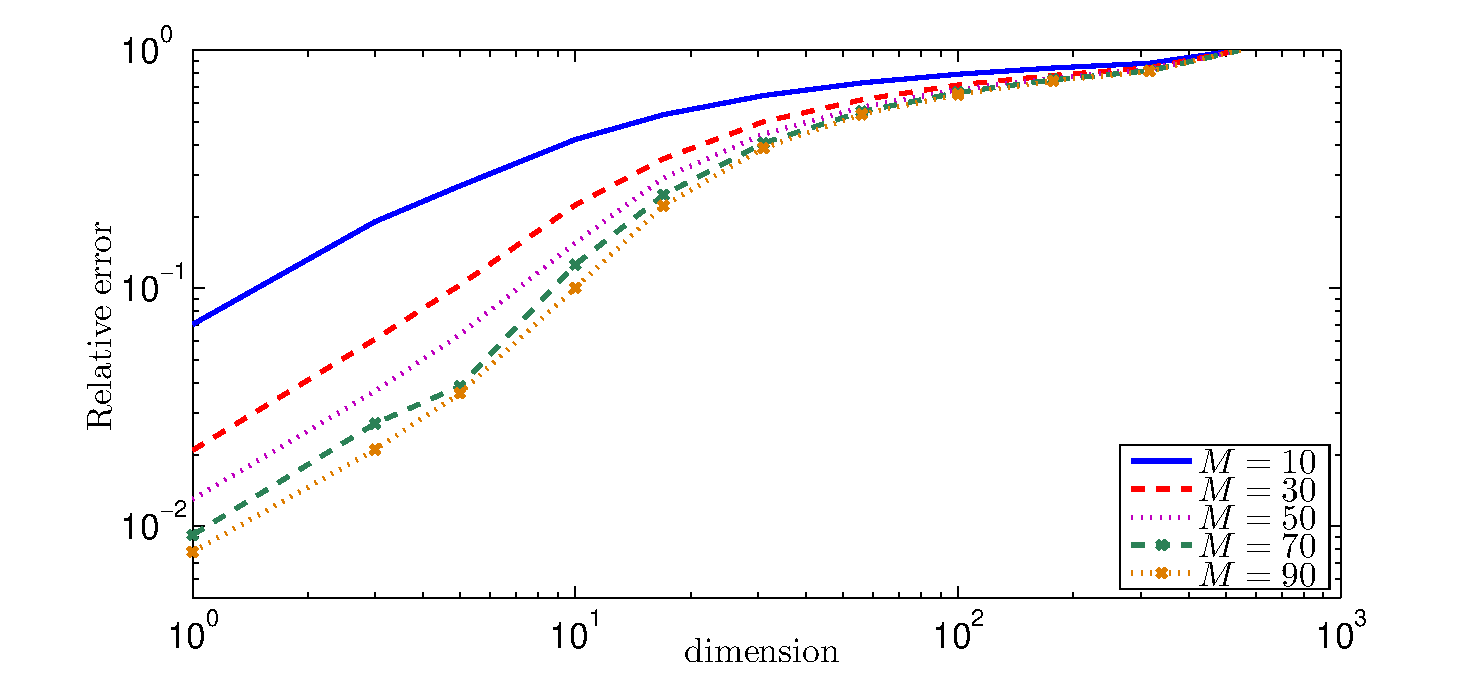
\includegraphics[width=\textwidth]{figures/ET_dim_scaling}
%\caption{Demonstration of the ETMC algorithm rapidly failing as the dimension increases. The relative error shown is that between the sampled mean and the true mean.}
%\label{fig:ET_dim_scaling}
%\end{center}
%\end{figure}

%Figure~\ref{fig:ET_dim_scaling} shows how quickly the ETMC algorithm loses its ability to accurately preserve the mean of the posterior distribution as the dimension increases. Clearly for a simple Gaussian problem, we can not resample in much more than 10 dimensions and hope to recover a representative sample, without hugely increasing the number of particles in the ensemble. As the cost of the ETMC is $\mathcal{O}(n^2)$, this does limit the dimension for which this approach can be used.

\subsection{Deficiencies of Metropolis-type MCMC schemes}
All MCMC methods are trivially parallelisable. One can take a method
and simply implement it simultaneously over a set of processes. All
of the states of all of the processes can be recorded, and in the time
that it takes one process to draw $N$ samples, $M$ processes can draw
$NM$ samples. 

However, we argue that this is a far from optimal
scenario. First of all, unless we have a lot of information about the posterior, we will begin the algorithm a long way from statistical equilibrium. Some initial iterations then are not samples from the posterior, and must be thrown away. This process is known as the burn-in. In a trivially parallelised scenario, each process must perform this process independently.

Moreover, many MCMC algorithms suffer from poor mixing, especially in
multimodal systems. The time for an MCMC trajectory to switch between modes can be
large and given that a large number of switches are required before we have a
good idea of the relative probability densities of these different
regions, it can be prohibitively expensive.

Another aspect of Metropolis-type samplers is that information
computed about a proposed state is simply lost if we choose to reject
that proposal in the Metropolis step. An advantage of importance
samplers is that no evaluations of $\mathcal{G}$ are ever wasted
since all samples are saved along with their relative weighting.

Moreover, a trivially parallelised MCMC scheme is exactly that -
trivial. Intuition suggests that we can gain some speed up by sharing information across the processes and that is
exactly what we wish to demonstrate in this paper.

These deficiencies of the trivial method of parallelising MCMC methods
motivated the development of the Parallel Adaptive Importance Sampler
(PAIS). In the next section we will introduce the method in its most
general form. We will then introduce the version that we have
implemented, which utilises the resampler recently suggested by
Reich\cite{reich2013nonparametric} described in Section
\ref{sec:filters}, and the pCNL proposal distribution described in
Section \ref{Sec:pCNL}


\section{The Parallel Adaptive Importance Sampler \allowbreak (PAIS)}\label{Sec:PAIS}

% In a trivially parallelised MCMC scheme, if we have enough processes
% all sampling from the target density at the same time, then we can
% make a very rough approximation of that density by taking the current
% states of all of the processes as a representative sample. In the
% PAIS, the proposal density for the importance sampler stage is a
% mixture of all of the proposal densities for a chosen MCMC scheme,
% using the current states. If the proposal in the MCMC scheme is
% appropriate and our number of samples is big enough, we might hope
% that this mixture of densities is a good enough approximation of the
% target density, and that new samples drawn from
% the mixture proposal are approximately draws from the target
% measure. If this is the case, then the variance of importance weights
% for these samples will be small, leading to a highly efficient
% sampler.

% The problem at this stage, is that our current states all have varying
% importance, but in order for us to iterate this whole process again,
% we require them to be the same. Therefore, we employ a resampler to
% take our new set of samples with differing weights, and return a set
% of states with equal weights, which are chosen so that the correlation
% between the two sets is maximised. At this stage we can start the whole
% process again. 

Important samplers can be a very efficient method for sampling from a
probability distribution. A proposal density is chosen from which we
can draw samples, and each sample is assigned a weight given by the
ratio of the target density and the proposal density at that
point. They are efficient when the proposal density is concentrated in
similar areas to the target density, and incredibly inefficient when
this is not the case. The aim of the PAIS is to use the states of a
set of parallel MCMC chains to construct a proposal distribution which
will be as close as possible to the target density. Given enough
processors, the states of all of these chains at one point
in time may be reasonably representative sample of the target density.

The proposal distribution could be constructed in many different ways,
but we choose to use a mixture distribution, made up of MCMC proposals
(in this paper, specifically the pCNL proposal from Section \ref{Sec:pCNL}). Once the proposal is
constructed, we can sample a new set of states from the proposal
distribution, and each is assigned a weight given by the ratio of the target
density and the proposal mixture distribution density. Assuming that
our proposal distribution is a good one, then the variance of the
weights will be small, and we will have many useful samples. Finally, we
need to create a set of evenly weighted samples which best represent
this set of weighted samples. This is achieved by implementing the
ETMC algorithm. Once we once again have a set of evenly weighted
samples that we believe represents the target distribution well, we
can iterate the process once again. The algorithm is given in more detail in Table \ref{tab:PAIS}. 

We wish to sample states $x \in X$ from a posterior
probability distribution $\mu_Y$. Since we have $M$ processes, we
represent the current state of all of the Markov chains as a vector
$\X = [x_1,x_2,\ldots,x_M]^T$. We are also given a transition kernel
$\nu(\cdot,\cdot)$, which might come from an MCMC method, for example
the pCNL proposal presented in Section \ref{Sec:pCNL}.

\begin{table}
\begin{mdframed}
\begin{algorithmic}
\STATE $\X^{(0)} = \X_0 = [x_1^{(0)},x_2^{(0)},\ldots,x_M^{(0)}]^T$
\FOR{$i=0,1,2, ..., N$}
\STATE $\Y^{(i)} = [y_1^{(i)},y_2^{(i)},\ldots,y_M^{(i)}]^T, \quad y_j^{(i)} \sim
\nu(\cdot;x_j^{(i)})$
\STATE $\chi(y;\X^{(i)}) = \frac{1}{M}
\sum_{j=1}^M \nu(y;x_j^{(i)})$.
\STATE $\W^{(i)} = [w_1^{(i)},w_2^{(i)},\ldots,w_M^{(i)}]^T,$ \quad $w^{(i)}_j =
\frac{\pi(y_j^{(i)})}{\chi(y_j^{(i)};\X^{(i)})}$.
\STATE Resample using ETMC: $(\W^{(i)},\Y^{(i)}) \rightarrow (\frac{1}{M}\mathbf{1}, \X^{(i+1)})$
\ENDFOR 
\end{algorithmic}
\end{mdframed}

\caption{A pseudo-code representation of the Parallel Adaptive
  Importance Sampler (PAIS).}
\label{tab:PAIS}
\end{table}

Since the resampling does not give us a statistically identical sample
to that which is inputted, we cannot assume that the samples $\X^{(i)}$
are samples from the posterior. Therefore, as with serial
importance samplers, the weighted samples
$(\W^{(i)},\Y^{(i)})_{i=1}^N$, or their statistics, are stored.

The key here is to choose a suitable transition kernel $\nu$ such that
if $X^{(i)}$ is a decent representative sample of the posterior,
the mixture density $\chi(\cdot;\X^{(i)})$ is a reasonable
approximation of the posterior distribution. If this is the case,
the newly proposed states $\Y^{(i)}$ will also be a good (and relatively
independent) sample of the posterior with low variance in the
weights $\W^{(i)}$.

In Section \ref{Sec:Num}, we will demonstrate how the algorithm
performs, using pCNL algorithm. We do not claim that this choice is optimal, but
is simply chosen as an example to show that sharing information across
processes can improve on the original MCMC algorithm and lead to
convergence in fewer evaluations of $\G$. This is important since if
the inverse problem being tackled involves computing
the likelihood from a very large data set this could lead to a
large saving of computational cost.

\section{Automated tuning of Algorithm Parameters}\label{Sec:adapt}

Efficient selection of scaling parameters in MCMC algorithms is critical to achieving optimal mixing rates and hence achieving fast convergence to the target density. One significant difficulty is finding an appropriate $\nu$ such that
$\chi$ is a close approximation to the posterior density $\pi$. If the proposal distribution is over-dispersed, then the algorithm will propose states a long way from the current state at the cost of a relatively low acceptance rate, impacting the quality of inferences on the posterior. Similarly, if the posterior is under-dispersed, the process will take a long time to fully explore the space so the mixing rate, and hence convergence rate, will be slow. It is therefore necessary to find a proposal distribution which is slightly over-dispersed to ensure the entire posterior is explored\cite{gelman1992inference}, but is as close to the posterior as possible.

Proposal distributions which are slightly over-dispersed as described
above, can be found by tuning the variance of the proposal
distribution $\nu$ during the burn-in phase of the
algorithm. Algorithms which use this method to find optimal proposal
distributions are known as adaptive MCMC algorithms. Adaptive MCMC
algorithms will converge to the stationary distribution $\pi(\cdot)$,
irrespective of whether the adaptive parameter itself converges to an
optimal value, under the following
conditions\cite{roberts2007coupling,roberts2009examples}: 
\begin{enumerate}
\item The adaptive parameter exhibits diminishing adaptation, which says that the amount of movement in the adaptive parameter decreases with the length of the chain. 
\item The smallest number of steps for which the kernel has sufficiently converged, from an initial state $x$, is finite, by bounded convergence.
\end{enumerate}

The variance of the proposal distributions that are used within the
proposal mixture distribution plays a key role in how well the
proposal distribution represents the target distribution, and
therefore how quickly the algorithm converges. A large over-dispersed
proposal distribution will sample a lot from the tails of the
distribution, but may also find other regions of high density with
respect to the target distribution. A very small variance in the
proposal distributions will lead to a very rough proposal mixture
distribution. In practise, we wish to find the happy medium in which
the proposal distribution is slightly more dispersed than the target
density, whilst also being a good representation of the regions which
have high density with respect to the target distribution.

Adaptively choosing the variance of the proposal distributions with a
large initial guess allows us to first explore the state space
globally, searching for multiple modes. Reducing the proposal variances to an
optimal value then allows us to explore each region efficiently. The
fact that we have multiple chains allows us to assess quickly and
effectively what the optimal variance of the proposal distributions
should be. 

In many MCMC algorithms such as the Random Walk Metropolis-Hastings (RWMH) algorithm, the optimal scaling parameter can be found by searching for the parameter value which gives an optimal acceptance rate, e.g. for near Gaussian targets we have 23.4\% for RWMH and 57.4\% for MALA\cite{roberts2001optimal}. Unlike Metropolis-Hastings algorithms, the PAIS algorithm does not accept or reject proposed values, so we need another method of measuring the optimality of $\delta$. Section~\ref{sec:statistics} gives some possible methods of tuning $\delta$.

\subsection{Statistics for Determining the Optimal Scaling Parameter}\label{sec:statistics}

\subsubsection{Determining optimal scaling parameter $\delta$ using error analysis}

MCMC algorithms can be assessed by comparing their approximation of the posterior to the analytic distribution. To assess this, a distance metric must be chosen. Examples are the relative error between the sample moments and the true moments, or the relative L2 error between the true density, $\pi(x|D)$, and the constructed histogram. The relative error in the $m$-th moment is
\[
	\left|\frac{N^{-1}\sum_{i=1}^N \! x_i^m - \mathbb{E}[X^m]}{\mathbb{E}[X^m]}\right|,
\]
where $\{x_i\}_{i=1}^N$ is a sample of size $N$ produced by the algorithm. The relative L2 error between a continuous function to a piecewise constant function, $e$, is
\begin{equation}\label{eqn:L2_error}
	e^2 = \sum\limits_{i=1}^{n_b}\left[\displaystyle\int_{R_i} \! \pi(a|D) \, \mbox{d}a - vB_i\right]^2 \Big/ \sum\limits_{i=1}^{n_b}\left[\displaystyle\int_{R_i} \! \pi(a|D) \, \mbox{d}a\right]^2,
\end{equation}
where the points $\{R_i\}_{i=1}^{n_b}$ are the $d$-dimensional histogram bins, so that $\bigcup_i R_i \subseteq X$ and $R_i\cap R_j=\emptyset$, $n_b$ is the number of bins, $v$ is the volume of a bin, and $B_i$ is the value of the $i$th bin. 

These statistics are not practical for finding optimal values of
$\delta$ since they require knowledge of the analytic solution, and
require that the algorithm be run for a long time to build up a
sufficiently large sample. However they can be used to assess the
ability of other statistical measures to find the optimal proposal
variances in a controlled setting.

Another related statistic, is the variance of the sample estimate of the first moment $\hat{\mu}$. Assuming that the algorithm is converging to the invariant distribution, convergence will be fastest when the variance of the estimate is minimised. This fact follows from the convergence rate of Monte Carlo algorithms, $\sigma/\sqrt{n}$. The proposal distribution which minimises the variance, $\sigma^2$, of $\hat{\mu}$, is the most desirable. This variance statistic often converges faster than the moment itself, and does not require any knowledge of the true value of the moment.

The following statistics can be used for importance sampling algorithms.

\subsubsection{Determining optimal $\delta$ using the variance of the weights}

Importance samplers assign a weight to each sample they produce, based on a ratio of the posterior to the proposal at that point. This type of sampler is most efficient when the posterior is proportional to the proposal distribution, in this case the weights are constant, and so the variance of the weights, $var(w(y))$, is zero. Hence, the optimal value of $\delta$, is
\[
	\delta^*_{\text{var}} = \arg\min_{\delta} \text{var}(w(y)).
\]
The mean of the estimator $\text{var}(w(y))$ is a smooth function, and so it is used to tune $\delta$ during the burn-in phase of MCMC algorithms. The variance of the estimator can be large, especially far away from the optimal value, so it can take a large number of samples to calculate descent directions.

\subsubsection{Determining optimal $\delta$ using the effective sample size}\label{sec:ess}

The effective sample size, $\neff$, can be used to assess the efficiency of importance samplers. Ideally, in each iteration, we would like all $M$ of our samples to provide us with new information about the posterior distribution. In practise, we are unlikely to achieve a ratio of exactly 1.

The effective sample size can be defined in the following way:
\[
	\neff = \frac{\left(\sum_{i=1}^M \! w_i\right)^2}{\sum_{i=1}^M \! w_i^2} \approx \frac{M\E(w)^2}{\E(w^2)} = M\left(1 - \frac{\mbox{var}(w)}{\mathbb{E}(w^2)}\right).
\]
The second two expressions are true when $M\rightarrow\infty$. From
the last expression we see that when the variance of the weights is
zero, $\neff = M$; this is our ideal scenario. In a neighbourhood around $\delta_{\text{var}}^*$, $\neff$ decreases when the variance increases. So if $v(w(y))$ can be equal to zero for a particular problem and proposal distribution, maximising the effective sample size is equivalent to minimising the variance of the weights. In the PAIS algorithm we have a dynamic proposal which is perturbed at every iteration.

The statistic $\neff$ converges faster than the variance of the weights, and so is preferable as a means of tuning $\delta$. While $\delta_{\text{var}}^*$ and the optimal value found using the effective sample size, $\delta_{\text{eff}}^*$, coincide when $v(w(y)) = 0$, this is not usually possible, so the methods will find different optimal values of $\delta^*$.

The $\neff$ statistic also has another useful property; if we imagine the algorithm in the burn-in phase, for example, we have $M$ processes in the tail of a Gaussian curve searching for the area of high density. If the processes are evenly spaced, then the particle closest to the mean will have an exponentially higher weight assigned to it. The effective sample size in this scenario will be close to 1. As the algorithm burns in, the processes find the flatter area near the mean so the number of samples contributing information to the posterior will increase. By this argument we can see that rising $\neff$ signals the end of the burn-in period.

\subsubsection{Behaviour of the effective sample size for varying ensemble size}

\begin{figure}[htpb]
\begin{center}
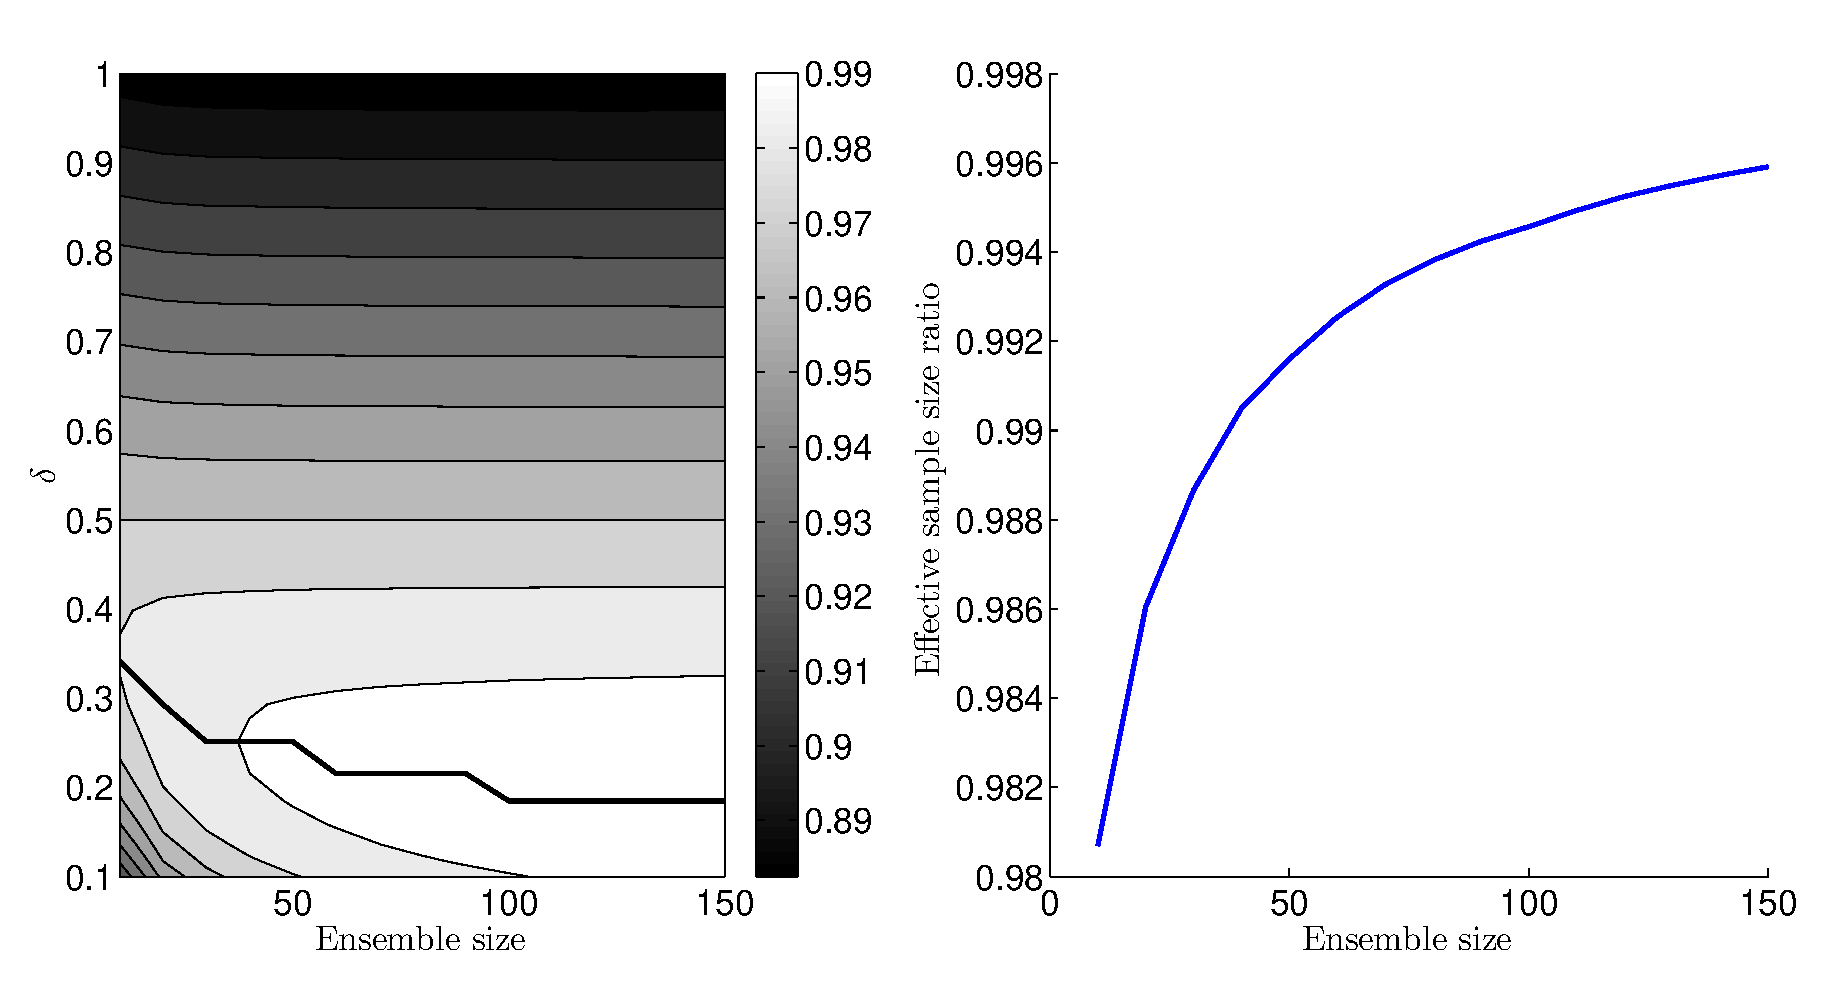
\includegraphics[width=\textwidth]{figures/neff-M}
\caption{Left: A contour plot showing how $\delta_{\text{eff}}$ varies with the ensemble size. The black line highlights the optimal value of $\delta$. Right: The value of the effective sample size ratio for the optimal $\delta$ at each ensemble size. i.e. the value of the effective sample size ratio along the black line in the left figure. Set up for this problem is given in Section~\ref{sec:problem 2}.}
\label{fig:neff-M}
\end{center}
\end{figure}

If we are to use the effective sample size ratio as an indicator of
how to tune the proposal variance, we need to look at how it behaves
in different situations. In Section \ref{Sec:Num} we see how it behaves for different observation operators. Here we look at how the statistic behaves as we vary the ensemble size, $M$. Figure~\ref{fig:neff-M} shows results for the second problem discussed in \ref{sec:problem 2} when using the PAIS-pCNL algorithm to explore the posterior distribution. The left part of the figure shows that as the ensemble size increases, the value of $\delta$ which gives the optimal effective sample size ratio decreases. This is to be expected since we are trying to fit more kernels into the posterior distribution, so the variance of each kernel needs to be decreased.

\subsection{The Adaptive Algorithm}\label{sec:adapt}

A popular approach for adaptive MCMC algorithms is to view the scaling
parameter as a random variable which we can sample during the course
of the MCMC iterations. However, it can be slow to converge to the
optimal value, and we may need an
uninformative prior for the scaling parameter. Alternatively, the parameter may be randomly sampled from some interval at various points during the chain, a benefit being that it allows some exploration of the state space but never converges to an optimal value of the scaling parameter. We choose to use a divide and conquer scheme which optimises the effective sample size. Some more sophisticated examples are described in \cite{roberts2009examples} and \cite{Ji2013adaptive}. The proposed algorithm, is not presented as an optimal strategy but as an example of the benefits of tuning the algorithm using the effective sample size statistic.

From hereon in, we will assume that we are using the proposal from the
pCNL algorithm given in Section \ref{Sec:pCNL}, which is given by:
\begin{equation}Y = (2+\delta)^{-1}\left[(2 - \delta)X_{i-1}-
2\delta\mathcal{C}\nabla \Phi(u)+
\sqrt{8\delta} W\right], \qquad W \sim \mu_0,
\end{equation}
where $X$ is our current state and $Y$ is our proposed state. The
scaling parameter $\delta$ dictates the variance in the proposal distribution.

 In the adaptive algorithm described in Table~\ref{tab:adapt} in
 Appendix \ref{Sec:App}, we calculate a sequence $\{\delta^{(k)}\}_{k=1}$ which converges to the optimal scaling parameter $\delta^*$, resulting in the optimal transition density $\chi$ for our MCMC algorithm. We must choose some sequence of iterations at which to update $\delta^{(j)}$, $\{n_k\}_{k=1}$, which can be decided using a sequence in which the terms grow exponentially further apart. The algorithm is given for the PAIS method but a similar method is used to adaptively calculate $\delta^*$ for the pCNL algorithm.

When implemented, there are a number of parameters which must be
chosen to allow efficient tuning of $\delta$. Firstly, the initial
value of $\delta$ should be chosen so that the chains spread out
quickly across the state space. However, if it is chosen to be too
large, then the method may become unstable and inefficient. We also choose two iteration numbers at which we change our adaptive strategy. At iteration $N_\text{join}$ we resample using the full ensemble size instead of using to subsets of the full ensemble. This allows us to fine-tune the scaling parameter using the full resampler, but slows down the rate of convergence of the scaling parameter. Finally we choose a time, $N_\text{stop}$, at which we stop updating our parameter to guarantee ergodicity of the MCMC algorithm.

\section{Numerical Examples}\label{Sec:Num}

\subsection{Sampling from a one dimensional Gaussian distribution}\label{sec:problem 1}

In this example we look at how PAIS compares to naively parallelised
MCMC. We compare the pCNL algorithm \cite{cotter2013mcmc} with its
PAIS variant, the PAIS-pCNL algorithm. We consider several statistics
for measuring the efficiency of the PAIS algorithm compared to
existing Metropolis-Hastings algorithms when applied to a simple one
dimensional Gaussian posterior.


Since we are comparing against trivially parallelised MCMC algorithms,
we also need to decide which statistic $T(\delta)$ to optimise for
these approaches. In the examples which follow, we have optimised the naively parallelised pCNL algorithm using the optimal acceptance rate $\hat{\alpha} = 0.75$. This value was found by using the L2 error minimums to calculate $\delta^*$. This means that we are minimising the statistic
\[
	T_{\text{MH}}(\delta) = \left| \frac{N_{\text{acc}}(\delta)}{N_{\text{total}}} - \hat{\alpha} \right|,
\]
where $N_{\text{acc}}(\delta)$ is the number of accepted moves and
$N_{\text{total}}$ is the total number of samples produced. For the
PAIS algorithm, we are maximising the effective sample size as
discussed in Section~\ref{sec:ess}, so $T_{\text{PAIS}}(\delta) =
\neff(\delta)$.

\subsubsection{Target distribution}

Consider the simple case of a linear observation operator $\G(u) = u$, where the prior on $u$ and the observational noise follow Gaussian distributions. Then, following Equation~\ref{eqn:like}, the Gaussian posterior has the resulting form
\begin{equation}\label{eqn:Gaussian posterior}
	\text{law}(\mu_Y) = \pi(u|D) \propto \exp\left(-\frac{1}{2}\big\|u - D\big\|^2_\Sigma - \frac{1}{2}\big\|u\big\|^2_{\mathcal{T}}\right),
\end{equation}
where $\Sigma$ and $\mathcal{T}$ are the covariances of the
observational noise and prior distributions respectively. In the
numerics which follow, we choose $\Sigma = \sigma^2I_N$ and
$\mathcal{T} = \tau^2I_d$ with $\tau^2 =2$ and $\sigma^2 = 0.1$, and
we observe $u=-2.5$ noisily such that
\[
D = \mathcal{G}(u) + \eta \sim \mathcal{N}(\mathcal{G}(u),\Sigma).
\]
These values result in a posterior density in which the vast majority
of the density is contained inside the high density region of the
prior. This means that it should be straightforward for the algorithm
to find the stationary distribution. The Kullback-Leibler (KL)
divergence, which gives us a measure of how different the prior and
posterior are, is $D_{KL}(\mu_Y || \mu_0) = 2.67$ for this problem.

\subsubsection{Numerical implementation}\label{sec:Implementation P1}

In each of the following simulations, we perform three tasks. First we calculate the optimal value of $\delta$ by optimising the statistics described in Section~\ref{sec:statistics}. Once we have these parameters, we run the algorithms and compare the convergence speeds of the algorithms. Finally, we implement the adaptive algorithms described in Section~\ref{sec:adapt} and compare the convergence of these algorithms with the nonadaptive algorithms.

{\bf (1) Finding the optimal parameters}: To find the optimal
parameters we choose 32 values of $\delta$ evenly spaced on a log scale
between $[10^{-5}, 2]$. We run the PAIS-pCNL algorithm for 10,000 iterations and pCNL for 100,000 iterations, each with $M=50$ processes. We took 32 repeats of both algorithms and then used the medians of the statistics to find the optimal parameters.

{\bf (2) Measuring convergence of nonadaptive algorithms}: We run the algorithms in Section~\ref{sec:problem 1} and Section~\ref{sec:problem 2} for 10 million iterations, again with 50 processes. The algorithms are run using the optimal parameters found in (1). The relative L2 error (Equation~\ref{eqn:L2_error}) is used as a measure of accuracy. The simulation for each algorithm was repeated 24 times.

{\bf (3) Measuring convergence of adaptive algorithms}: We run the
adaptive algorithms under the same conditions as the nonadaptive
algorithms, and again use the relative L2 error to compare
efficiency. The initial value of $\delta$ is given in the discussion
of each simulation.


\subsubsection{Optimal values of $\delta$}\label{sec:Optimal values P1}

\begin{figure}[htb]
\centering
\includegraphics[width=0.45\textwidth]{"figures/pCNL1o"}
\includegraphics[width=0.45\textwidth]{"figures/PAISpCNL1o"}
\caption{Finding optimal values of $\delta$ for the pCNL (left) algorithm and PAIS-pCNL (right) algorithm for the problem in Section~\ref{sec:problem 1}. The setup is as in Section~\ref{sec:Implementation P1}.}
\label{fig:P1 opt delta}
\end{figure}

\begin{table}[!htb]
    \begin{minipage}{.5\linewidth}
      \centering
        \begin{tabular}{|c|r|}
	\hline
	Statistic											& pCNL \\ \hline
	$\delta_{\text{L2}}^*$								& 3.7e-3 \\
	$\delta_{\text{var}(\hat{\mu})}^*$					& 5.8e-2 \\
	Acceptance Rate ($\delta_{\text{L2}}^*$)				& 9.9e-1 \\
	Acceptance Rate ($\delta_{\text{var}(\hat{\mu})}^*$)	& 7.4e-1 \\
	\hline
	\end{tabular}
    \end{minipage}%
    \begin{minipage}{.5\linewidth}
      \centering
        \begin{tabular}{|l|r|r|}
	\hline
	Statistic							& PAIS-pCNL \\ \hline
	$\delta_{\text{eff}}^*$				& 1.5e-2 \\
	$\delta_{\text{var}(w(y))}^*$		& 6.4e-2 \\
	$\delta_{\text{L2}}^*$				& 1.7e-2 \\
	\hline
	\end{tabular}
    \end{minipage}
	\caption{Optimal values of $\delta$ summarised from Figure~\ref{fig:P1 opt delta}. Statistics calculated as described in Section~\ref{sec:statistics}.}
	\label{table:prob1 opt delta}
\end{table}

Figure~\ref{fig:P1 opt delta} (left) shows the two values of $\delta$ which may be optimal for the pCNL algorithm, found at the turning points. The first estimate comes from the relative L2 error, and the second comes from the variance of the estimate of the mean. The optimal acceptance rates of the function space algorithms are expected to be slightly higher than their finite dimensional versions. Since the L2 error estimate of the histogram gives an acceptance rate which is near to 100\%, we say that the optimal acceptance rate is that as given by the variance of the mean, roughly 75\%. The results in Figure~\ref{fig:P1 opt delta} are summarised in Table~\ref{table:prob1 opt delta} (left).

Figure~\ref{fig:P1 opt delta} (right) shows the effective sample size ratio compared to the error analysis and the variance of the weights. Although the L2 error graph is noisy, the maximum in the effective sample size is close to the minimum in the L2 error. The minimum in the variance of the weights however is a long way away. We choose the effective sample size as the best estimator of the optimal scaling parameter because of this, and because the effective sample size statistic converges to a smooth graph faster than either the variance of the weights or the L2 error.

\subsubsection{Convergence of pCNL vs PAIS-pCNL}

\begin{figure}[htb]
\centering
\includegraphics[width=0.45\textwidth]{"figures/pCNL1l"}
\includegraphics[width=0.45\textwidth]{"figures/pCNL1m"}
\caption{Relative error in the first moment (right) and histograms (left) produced by the (A)pCNL and (A)PAIS-pCNL algorithms against iterations for problem~\ref{sec:problem 1}. The setup is as in Section~\ref{sec:Implementation P1} (2, 3).}
\label{fig:MH1 L2}
\end{figure}

Figure~\ref{fig:MH1 L2} shows that the PAIS-pCNL algorithm converges to the posterior distribution faster than the standard function space pCNL algorithm, in both L2 error and relative error in the moments. A description of the speed up attained by this algorithm is given in Section~\ref{sec:calc_saving}.

Both adaptive algorithms are run with initial values of $\delta_0=0.1$. From Figure~\ref{fig:MH1 L2} we can see that the APAIS-pCNL algorithm converges at least as quickly as the PAIS-pCNL algorithm. The ApCNL algorithm initially has trouble converging to the posterior; during the initial burn-in phase, some chains find themselves a long way out in the tails where due to the high gradient they will overshoot the high density region and reject almost all proposed values.

\subsubsection{Scaling of the PAIS algorithm with ensemble size}

Throughout this paper, we use an ensemble size $M=50$, but it is interesting to see how the PAIS algorithm scales if we were to increase the ensemble size, and if there is some limit below which the algorithm fails. We implement the problem in Section~\ref{sec:problem 1}, using the pCNL algorithm with ensemble sizes ranging from $M=2$ up to $M=494$.

\begin{figure}[h]
\begin{center}
\includegraphics[width=\textwidth]{"figures/PAIS_saving"}
\caption{Ratio of PAIS-pCNL samples required to reach the same tolerance as the pCNL algorithm.}
\label{fig:PAIS_saving}
\end{center}
\end{figure}

Figure~\ref{fig:PAIS_saving} was produced using the method of finding
optimal $\delta$ described in Section~\ref{sec:Implementation P1}(1),
then running 32 repeats at each ensemble size. The convergence rates
are then found by regressing through the data. The graph is still very
noisy but demonstrates that increasing the ensemble size continues to
reduce the number of iterations required in comparison with naive
MCMC. When $M<8$, the algorithm takes a long time to reach
stationarity. This indicates superlinear improvement of PAIS with
respect to ensemble size, in terms of the number of iterations
required, which is a demonstration of our belief that parallelism of
MCMC should give us added value over and above that provided by naive parallelism.

\subsection{Sampling from a one dimensional Gaussian with a higher KL divergence}\label{sec:problem 2}

In this example we use the same setup used in Section~\ref{sec:problem 1}. We choose a posterior distribution which has most of its mass far out in the tails of the prior distribution. The KL divergence is $D_{KL}(\mu_Y||\mu_0) = 4.670$. This means that the algorithm will have to ``work harder'' to find the area of high probability in the posterior density.

\subsubsection{Target distribution}

As in the previous example, we use the identity observation operator
$\G(u)=u$, which results in the Gaussian posteriors in
Equation~\ref{eqn:Gaussian posterior}. However, this time we choose
$\sigma^2=0.01$ and $\tau^2=0.01$ so the posterior distribution is
$\N(D/(1+\sigma^2/\tau^2), \tau^2\sigma^2/(\sigma^2+\tau^2)) = \N(D/2,
0.005)$ which for large $D$ is a long way out in the tail of the prior
with a very small variance. For the simulations which follow we
observe a reading of $u=4$, with observational noise drawn from $\N(0, \sigma^2)$.

\subsubsection{Optimal values of $\delta$}

\begin{figure}[htb]
\centering
\includegraphics[width=0.45\textwidth]{"figures/pCNL2o"}
\includegraphics[width=0.45\textwidth]{"figures/PAISpCNL2o"}
\caption{Finding optimal values of $\delta$ for the pCNL (left) algorithm and PAIS-pCNL (right) algorithm for the problem in Section~\ref{sec:problem 2}. The setup is as in Section~\ref{sec:Implementation P1}.}
\label{fig:P2 opt delta}
\end{figure}

\begin{table}[!htb]
    \begin{minipage}{.5\linewidth}
      \centering
        \begin{tabular}{|c|r|}
	\hline
	Statistic											& pCNL \\ \hline
	$\delta_{\text{L2}}^*$								& 8.6e-2 \\
	$\delta_{\text{var}(\hat{\mu})}^*$					& 9.1e-1 \\
	Acceptance Rate ($\delta_{\text{L2}}^*$	)			& 9.9e-1 \\
	Acceptance Rate ($\delta_{\text{var}(\hat{\mu})}^*$)	& 8.1e-1 \\
	\hline
	\end{tabular}
    \end{minipage}%
    \begin{minipage}{.5\linewidth}
      \centering
        \begin{tabular}{|l|r|r|}
	\hline
	Statistic							& PAIS-pCNL \\ \hline
	$\delta_{\text{eff}}^*$				& 2.6e-1 \\
	$\delta_{\text{var}(w(y))}^*$		& 2.6e-1 \\
	$\delta_{\text{L2}}^*$				& 2.8e-1 \\
	\hline
	\end{tabular}
    \end{minipage}
	\caption{Optimal values of $\delta$ summarised from Figure~\ref{fig:P2 opt delta}. Statistics calculated as described in Section~\ref{sec:statistics}.}
	\label{table:P2 opt delta}
\end{table}

We find the optimal values of $\delta$ using the same methods described in Sections~\ref{sec:Implementation P1} and \ref{sec:Optimal values P1}. The results are displayed in Figure~\ref{fig:P2 opt delta} and Table~\ref{table:P2 opt delta}. There is a huge difference between the two error estimates of $\delta$ for pCNL, although the corresponding variance graph is very flat making it sensitive to Monte Carlo error. The variance of the mean estimate has an 81\% acceptance rate, which is larger than the pCNL acceptance rate found previously.

For the PAIS-pCNL algorithm, it is again clear that the effective sample size ratio is a useful statistic for judging the optimal value of $\delta$. The relative L2 error estimate of $\delta^*$, shown in Table~\ref{table:P2 opt delta}, is slightly higher than the other two estimates, but from the graph there again seems to be a fairly flat wide minimum which is in the same region as the optimal effective sample size ratio. The variance of the weights becomes so small in the critical region that we get numerical zeroes, which means that we could not use this method to tune the scaling parameter adaptively.

\subsubsection{Convergence of pCNL vs PAIS-pCNL}

\begin{figure}[htb]
\centering
\includegraphics[width=0.45\textwidth]{"figures/pCNL2l"}
\includegraphics[width=0.45\textwidth]{"figures/pCNL2m"}
\caption{Relative error in the first moment (right) and histograms (left) produced by the (A)pCNL and (A)PAIS-pCNL algorithms against iterations for problem~\ref{sec:problem 2}. The setup is as described in Section~\ref{sec:Implementation P1} (2,3).}
\label{fig:MH2 L2}
\end{figure}

Figure~\ref{fig:MH2 L2} shows that the PAIS-pCNL algorithm, converges to the posterior distribution faster than the pCNL algorithm. The adaptive algorithms both struggle with the first moment for the first million iterations, but produce better estimates after 10 million iterations. 

\subsection{Sampling from Bimodal Distributions}

In this section we investigate the behaviour of the PAIS algorithm
when applied to bimodal problems. Metropolis-Hastings methods can
struggle with multimodal problems, particularly where switches between
the modes are rare, resulting in incorrectly proportioned modes in the
histograms, for example. With the PAIS algorithm, we see that the
resampling step redistributes chains to new modes as they are
found. This means that we expect the number of chains in a mode to be
approximately proportional to the probability mass in that mode. As a result, reconstructed posteriors with disproportional modes, as is familiar with the Metropolis-Hastings algorithms, are not produced. We again look at an `easy' problem, BM(1), which has a KL divergence of 0.880, and a `harder' problem, BM(2), which has a KL divergence of 3.647. Problem BM(1) has two modes which are separated by a smaller energy barrier. In BM(2) we increase the distance between the two modes which has the effect of increasing the required energy to jump between modes. These posteriors are shown in Figure~\ref{fig:problem 3 posteriors}.

\subsubsection{Target Distribution}

The following setup is the same for both problems. We consider an observation operator $\G(u) = u^2$, and assign the prior $u \sim \mu_0 = \N(0, \tau^2=0.25)$. We assume that a noisy reading, $D$, is taken according to $D = \G(u) + \varepsilon$, where $\varepsilon \sim \mu_\varepsilon = \N(0, \sigma^2 = 0.1)$. This results in the non-Gaussian posterior
\[
	\pi(u|D) \propto \exp\left(-\frac{1}{2\sigma^2}\|u^2 - D\|^2 - \frac{1}{2\tau^2}\|u\|^2\right).
\]
To create the `easy' problem we say that the true value of $\G(u) = 0.75$, and the `hard' problem is generated using $\G(u) = 2$. In the numerics which follow we draw noise from $\mu_\varepsilon$ to generate our data point.

\begin{figure}[htpb]
\begin{center}
\includegraphics[width=\textwidth]{"figures/posteriors3"}
\caption{Posterior distributions for problem BM(1) and BM(2). Problem BM(1) has a noisy data value of  0.921312 which results in an energy barrier which is relatively easy to cross, as well as their common prior distribution.}
\label{fig:problem 3 posteriors}
\end{center}
\end{figure}

\subsubsection{Numerical Implementation}\label{sec:Implementation P2}

The numerical implementation for most of the following simulations follow the same setup as described in Section~\ref{sec:Implementation P1}. The only exception is that the convergence plots for both adaptive and nonadaptive algorithms are run for $10^6$ iterations instead of $10^7$.

\subsubsection{Calculating values of Optimal $\delta^*$}\label{sec:BM1_opt_delta}

Calculating the optimal values of the scaling parameters for this problem is similar to the Gaussian case; we check only the acceptance rate to find the optimal values for pCNL and we use the effective sample size to find the optimal values for PAIS-pCNL. Table~\ref{table:BM_opt_delta} gives the optimal values of $\delta$ for both problems.

\begin{table}[!htb]
    \begin{minipage}{.5\linewidth}
      \centering
        \begin{tabular}{|l|r|r|}
	\hline
	Algorithm							& $\delta^*_{\text{acc}}$	& $\delta^*_{\text{eff}}$ \\ \hline
	pCNL								& 1.9e-1					& - \\
	PAIS-pCNL							& -						& 3.9e-2\\
	\hline
	\end{tabular}
    \end{minipage}%
    \begin{minipage}{.5\linewidth}
      \centering
        \begin{tabular}{|l|r|r|r|}
	\hline
	Algorithm							& $\delta^*_{\text{acc}}$	& $\delta^*_{\text{eff}}$	& $\delta^*_{\text{L2}}$ \\ \hline
	pCNL								& 5.8e-2					& - 						& 9.1e-1\\
	PAIS-pCNL							& -						& 2.6e-2 					& 2.6e-2\\
	\hline
	\end{tabular}
    \end{minipage}
	\caption{Optimal values of $\delta$ for BM(1) (left) and BM(2) (right).}
	\label{table:BM_opt_delta}
\end{table}

In problem BM(1), the pCNL algorithm has the
higher value of $\delta$, which corresponds to a close to independence
sampling, effectively sampling from the prior. This is because the
regions with the majority of the target density are well covered by
the prior. The PAIS-pCNL algorithm samples more efficiently from its
mixture $\chi$, and so a lower value of $\delta$ is more efficient.

Problem BM(2) is much harder than BM(1); transitions between the modes
are extremely unlikely for the standard pCNL algorithm. This means that we need to consider the
convergence on two levels; we should consider the algorithm's ability
to find all the modes, and to sample them thoroughly and in the correct proportions.

To get correctly proportioned modes with the pCNL algorithm it is
important that the chains can transition between the modes, which
means that $\delta$ must be large. However, this leads to a lower
acceptance rate, and so we sacrifice convergence locally. The prior distribution $\mu_0$ is
not a good approximation of the posterior distribution, and so too
large a value of $\delta$ (which leads to an independence sampler
using the prior as a proposal distribution) leads to an inefficient
method sampling. For these reasons, the pCNL algorithm is very slow to
converge for problems of this type.

We can achieve these two regimes in pCNL by tuning $\delta$ using the acceptance rate for local convergence, and by L2 error for global convergence. Similarly in PAIS-pCNL we can use the effective sample size for local convergence, and the L2 error for global convergence.

From Table~\ref{table:BM_opt_delta} (right) we see that there is a large difference between the optimal value of $\delta$ for each regime, meaning that both will result in inefficient sampling. The PAIS-pCNL algorithm manages to sample the detail and the large scale behaviour with the same value of $\delta^*$: a clear advantage to using this algorithm for this problem.

\subsubsection{Convergence of pCNL vs PAIS-pCNL}

We see a significant speed with the PAIS-pCNL algorithm for BM(1). Figure~\ref{fig:BM1_L2} shows the adaptive and nonadaptive convergence rates. 

\begin{figure}[htpb]
\begin{center}
\includegraphics[width=\textwidth]{"figures/BM1_L2"}
\caption{Error analysis for the PAIS-pCNL and pCNL algorithms for
  problem BM(1). The solid blue line, and dashed red line compare the algorithms with fixed optimal scaling parameters, and the blue crossed and magenta crossed lines compare the adaptive algorithms. The setup is as described in Section~\ref{sec:Implementation P2} (2,3).}
\label{fig:BM1_L2}
\end{center}
\end{figure}

We can see that the adaptive algorithms compare closely with the
respective nonadaptive algorithms and the improvement PAIS offers
remains significant.

For BM(2) the algorithms are run with the global optimal value of $\delta^*$, and with the local optimal value of $\delta^*$. Figure~\ref{fig:BM2_L2} shows that the algorithms using the globally optimal $\delta^*$ convergence diagnostics converge slowly towards the true posterior after a long burn-in period, whereas the algorithms using the local optimal $\delta^*$ converge quickly, but get stuck in one mode meaning that the convergence rate flattens out.

\begin{figure}[h]
\begin{center}
\includegraphics[width=\textwidth]{"figures/BM2_L2"}
\caption{pCNL and PAIS-pCNL convergence statistics using locally and
  globally optimal $\delta$, for problem BM(2). The setup is as described in Section~\ref{sec:Implementation P2} (2).}
\label{fig:BM2_L2}
\end{center}
\end{figure}

The adaptive algorithm as stated in Section~\ref{sec:adapt} is one way of combining the two regimes. Another method uses a small number of `scout' chains with a large $\delta$ to continually search out new modes. Other methods of mode searches are described in \cite{lan2013wormhole}, and the regeneration method is applicable\cite{nummelin1984general}.

Figure~\ref{fig:BM2_AL2} shows the success of the (A)PAIS-pCNL algorithms in converging to the posterior, compared to the (A)pCNL algorithms. We can see that using the pCNL algorithm for this problem would be infeasible.

\begin{figure}
\begin{center}
\includegraphics[width=\textwidth]{"figures/BM2_AL2"}
\caption{Convergence graphs for problem BM(2), the (A)pCNL and (A)PAIS-pCNL algorithms have been run with optimal $\delta^*$ for the L2 error and the adaptive algorithm described in Section~\ref{sec:adapt}. The setup is as described in Section~\ref{sec:Implementation P2} (3).}
\label{fig:BM2_AL2}
\end{center}
\end{figure}

\subsubsection{Calculating the Speed Up in Convergence}\label{sec:calc_saving}

\begin{figure}
\begin{center}
\includegraphics[width=\textwidth]{"figures/calc_saving"}
\caption{Illustration of calculating the number of PAIS-pCNL iterations required to reach a tolerance of $10^{-2}$ as a percentage of pCNL iterations. The relative L2 error graphs are from the problem in Section~\ref{sec:problem 1}.}
\label{fig:calc_saving}
\end{center}
\end{figure}

The graphs in the previous section clearly show that the PAIS-pCNL algorithm converges faster than the pCNL algorithm when both are parallelised with the same number of threads. We can calculate the number of iterations required to achieve a particular tolerance level in our solution for each algorithm and compare these to calculate a percentage saving. In Figure~\ref{fig:calc_saving} we demonstrate our calculation of the savings. The constants $c_1$ and $c_2$ are found by regressing through the data with a fixed exponent of $-1/2$ excluding the intial data points where the graph has not finished burning in.

A summary of the percentage of iterations required using the PAIS algorithm compared with the respective Metropolis-Hastings algorithms is given in Table~\ref{table:calc_savings}. The blank entries correspond to occasions when the MH algorithms haven't converged to the posterior distribution.

\begin{table}[!h]
\centering
\begin{tabular}{|l|l|r|r|}
\hline
		& & Low KL div & High KL div \\ \hline
	\multirow{4}{*}{Gaussian}	&RWMH & 14\% & 14\% \\
	&pCN & 33\% & - \\
	&MALA & 41\% & 42\% \\
	&pCNL & 62\% & 66\% \\ \hline
	\multirow{4}{*}{Bimodal}	&RWMH & 40\% & 44\% \\
	&pCN & 32\% & - \\
	&MALA & 36\% & 40\% \\
	&pCNL & 56\% & - \\ \hline
\end{tabular}
\caption{Iterations for the PAIS algorithms required to achieve a desired tolerance as a percentage of the number of iterations required by the respective Metropolis algorithms.}
\label{table:calc_savings}
\end{table}

\subsubsection{A Useful Property of the PAIS Algorithm for Multimodal Distributions}

\begin{figure}[!h]
\begin{center}
\includegraphics[width=\textwidth]{"figures/BM2_suction"}
\caption{This figure demonstrates the redistribution property of the PAIS algorithm. Initially there is one chain in the positive mode, and 49 chains in the negative mode.}
\label{fig:BM2_suction}
\end{center}
\end{figure}

The biggest issue for the Metropolis-Hastings algorithms when sampling
from a posterior such as the one in BM(2) is that it is unlikely that
the correct ratio of chains will occur in each of the modes, and since there is no interaction between the chains, there is no way to remedy this problem. The PAIS algorithm tackles this problem with its resampling step. The algorithm uses its dynamic kernel to build up an approximation of the posterior at each iteration, and then compares this to the posterior distribution via the weights function. Any large discrepancy in the approximation will result in a large or small weight being assigned to the relevant chain, meaning the chain will either pull other chains towards it or be sucked towards a chain with a larger weight. In this way, the algorithm allows chains to `teleport' to regions of the posterior which are in need of more exploration. Figure~\ref{fig:BM2_suction} shows Problem BM(2) with initially 1 chain in the positive mode, and 49 chains in the negative mode. It takes only a handful of iterations for the algorithm to balance out the chains into 25 chains in each mode. The chains switch modes without having to climb the energy gradient in the middle.

\section{Discussion and Conclusions}\label{Sec:Conc} 

We have explored the application of parallelised MCMC algorithms in
low dimensional inverse problems. We have demonstrated numerically
that these algorithms converge faster than the analogous naively parallelised
Metropolis-Hastings algorithms. Further experimentation with the
Random Walk Metropolis-Hastings (RWMH), Metropolis Adjusted Langevin
Algorithm (MALA) and preconditioned Crank-Nicolson (pCN) proposals has
yielded similar results\cite{Paul}.%  Importantly, we have demonstrated
% that the convergence rate improves superlinearly with respect to the
% number of processors used.

Importantly, we have compared the efficiency of our parallel scheme
with a naive parallelisation of serial methods. Thus our increase in
efficiency is over and above an $N$-fold increase, where $N$ is the
number of cores or processors at our disposal. Our approach
demonstrates a better-than-linear speed-up with the number
processors/cores used. Thus, our approach is not only embarrassingly
parallel (as coined by Cleve Moler in \cite{moler1986matrix}), but
humiliatingly so.

The PAIS has a number of favourable features, for example the
algorithm's ability to redistribute, through the resampling regime,
the chains to regions which require more exploration. This allows the
method to be used to sample from complex multimodal distribution.

The PAIS approach is limited by the curse of dimensionality, since the
cost of the resampling algorithm becomes prohibitively large. The cost
of the resampler is $\mathcal{O}(n^2)$, where $n$ is the number of
particles in the ensemble. Other resamplers exist which are not as
costly, but for which there is some sacrifice in terms of optimality
of the output. For example, the resampler proposed in
\cite{schefzik2013uncertainty}  has computational complexity
$\mathcal{O}(n)$. This might allow the PAIS to be used in higher
dimensional problems, and is an avenue for future investigation.

Another strength of the PAIS is that it can also be used with any MCMC
proposal. There are a growing number of increasing sophisticated MCMC
algorithms (HMC, Riemann manifold MCMC etc) which could be incorporated into this framework, leading to
even more efficient algorithms, and this is another opportunity for
future work.

One disadvantage of parallelised algorithms is that often different
processors will complete their tasks in different amount of times, for
a number of reasons, often due to communication between the
processors. One approach which could be applied to the PAIS to avoid
this is for each processor to immediately start a new iteration, only
using the last values of the other processors that were communicated
to it. This incomplete approach would still be valid, and could lead
to more efficient use of the computer architecture.



\bibliographystyle{siam}
\bibliography{refs}

\begin{appendix}
\section{The adaptive PAIS algorithm}\label{Sec:App}
\begin{table}[!h]
\begin{mdframed}
\begin{algorithmic}
\STATE $x_j^{(0)} \sim \mu_0$, for $j \in L\cup U$, where $L = \{j\}_{j=1}^{M/2},\ U = \{j\}_{j=M/2+1}^M$.
\STATE Choose $\delta^{(1)} \in (0, 2]$. Set $\delta_{L,U}^{(1)} = (1\pm 0.01)\delta^{(1)}\wedge 2$.
\FOR{$i=1,2, \ldots, N$}
\STATE $y_j^{(i)}~\sim~Q(x_j^{(i-1)},\delta_L^{(i)})$ for $j \in L$, and $y_j^{(i)}~\sim~Q(x_j^{(i-1)},\delta_U^{(i)})$ for $j \in U$.
\STATE Calculate 
\[
	w^{(i)}_j = \frac{\pi(y_j^{(i)})}{\nu(y_j^{(i)};X^{(i-1)})},
\]
where
\[
	\nu(y;X) = \frac{1}{M}\sum_{j\in L} q(y;x_j,\delta_L)+\frac{1}{M}\sum_{j\in U} q(y;x_j,\delta_U).
\]

\IF{$i$ is in $\{n_k\}_{k=1}$}
	\STATE For $w_{kj} = w_j^{(k)}$, $S = n_k - n_{k-1}$,
	\STATE $T_L = SM(\sum_{k=i-S}^S\sum_{j\in L} w_{kj})^2/(\sum_{k=i-S}^S\sum_{j\in L} w_{kj}^2)$.
	\STATE $T_U = SM(\sum_{k=i-S}^S\sum_{j\in U} w_{kj})^2/(\sum_{k=i-S}^S\sum_{j\in U} w_{kj}^2)$.
	\STATE $\delta^{(i+1)} = \delta^{(i)} - \Delta t \displaystyle\frac{T_U - T_L}{\delta_U^{(i)}-\delta_L^{(i)}}$.
\ELSE
	\STATE $\delta^{(i+1)} = \delta^{(i)}$.
\ENDIF

\IF{$i < N_\text{stop}$}
	\IF{$i < N_\text{join}$}
		\STATE Resample 
	\[
		(w_j^{(i)},y_j^{(i)})_{j\in L} \rightarrow (\frac{1}{M}, x_j^{(i)})_{j\in L}, \quad (w_j^{(i)},y_j^{(i)})_{j\in U} \rightarrow (\frac{1}{M}, x_j^{(i)})_{j\in U}.
\]
	\ELSE
		\STATE Resample $(w^{(i)},Y^{(i)}) \rightarrow (\frac{1}{M}\mathbf{1}, X^{(i)})$.
	\ENDIF
	\STATE $\delta_{L,U}^{(i)} = \delta^{(i)} \pm 2\sqrt{2}\delta^{(i)}/\sqrt{NM} \wedge 2$.
\ELSE
		\STATE Resample $(w^{(i)},Y^{(i)}) \rightarrow (\frac{1}{M}\mathbf{1}, X^{(i)})$.
		\STATE $\delta_L^{(i+1)} = \delta_U^{(i+1)} = \delta^{(i+1)}$.
\ENDIF
\ENDFOR
\end{algorithmic}
\end{mdframed}\caption{A pseudo-code representation of the adaptive
  PAIS algorithm.}
\label{tab:adapt}
\end{table}
\end{appendix}

\end{document}
